\chapter{Anomaliedetektion}\label{ch:anomaliedetektion}
Anomaliedetektion beschreibt die Aufgabe, Trends, Muster und Punkte in einem Datensatz zu finden, die nicht dem Normalzustand
entsprechen~\cite{Chandola2009}. Anders gesagt lautet das Ziel: die Punkte finden, die sich von den anderen Punkten im Datensatz
stark unterscheiden~\cite[Kap.~10]{Tan2014}. Diese andersartigen Datenpunkte oder -sequenzen werden in der Regel als Anomalie,
Ausreißer oder Ausnahmen bezeichnet, wobei Anomalie der geläufigste Begriff ist. Anomaliedetektion findet große Verwendung in
verschiedenen Anwendungsbereichen, wie z.~B.~in der Netzwerktechnik zur Erkennung von potenziellen Angriffen durch Eindringlinge
in ein Netzwerk anhand von ungewöhnlichem Traffic~\Cite{Bernacki2015}. Auch in der Medizin können nach einem EKG durch
Anomaliedetektion Herzrhythmusstörungen erkannt werden~\cite{Chauhan2015}, genau wie eine Bank ein Interesse an Anomalien im
Kreditkartenverhalten ihrer Kunden hat, um Betrugsfälle zu erkennen~\cite{Jiang2023, CeronmaniSharmila2019}.

Die simpelste Herangehensweise zur Erkennung von Anomalien ist die, dass zuerst definiert wird, welche Punkte im Datensatz normalem
Verhalten entsprechen und alle davon abweichenden Punkte als Anomalie zu kennzeichnen. Doch so einfach die Herangehensweise wirkt,
so anfällig ist sie auch für Fehler. Dabei heben sich einige Herausforderungen hervor.

Zum Einen die Frage, wo genau die Grenze zwischen normalem und anomalem Verhalten liegen soll. Eine Region zu definieren, die jeden 
möglichen normalen Punkt beinhaltet und jedmöglichen anomalen Punkt ausschließt, ist nicht trivial und oft nicht präzise durchführbar.
So ist es durchaus möglich, dass in manchen Fällen anomale Punkte als normal bezeichnet werden, und normale Punkte als anomal, je
nachdem, wo die Grenze liegt.

Es stellt sich ebenfalls die Frage, ob eine Anomalie einer binären Natur unterliegt: Entweder es handelt sich um eine Anomalie oder
einen Normalzustand. Doch die Wahrheit liegt oft in der Mitte. Weicht ein Punkt oder eine Sequenz bereits nur leicht vom Normal ab,
so kann es bereits erste Hinweise auf mögliches zukünftiges anomales Verhalten geben, bevor solche Datenpunkte bereits als Anomalie
gekennzeichnet werden. Deshalb ist es ratsam, charakterisieren zu können, wie weit der Punkt oder die Sequenz vom Normal abweicht.
Diese Charakterisierung kann dabei als \textit{Anomaly Score} bezeichnet werden und beispielsweise eine Dezimalzahl zwischen 0 und 1
sein.

Normalzustände sind in Zeitserien oft zeitvariant und daher schwer festzuhalten bei einer kontinuierlichen Datenaufzeichnung.
Zudem sind Normalzustände und Abweichungen davon in unterschiedlichen Bereichen auch unterschiedlich signifikant. Während beim
menschlichen Körper eine geringe Abweichung der Körpertemperatur bereits gravierend sein kann, ist die gleiche relative Abweichung
in einer anderen Domäne wie in einem Aktienkurs weniger drastisch und unterliegt dementsprechend auch einem Anpassungsbedarf, bevor
es an die Erkennung möglicher Anomalien geht.

Daraus lässt sich direkt zum nächsten Problem übergehen. Die Unterscheidung zwischen globalen und lokalen Anomalien bzw.~allgemeiner
formuliert globale und lokale Ungewöhnlichkeiten, bevor sie als Anomalie aufgefasst werden. Hier ist der Kontext wichtig: Eine Person
mit einer Körpergröße von mehr als 2 $m$ ist in ihrer Nachbarschaft sicherlich eine Anomalie, während sie in einem Basketballteam
kaum herausragt~-~im wahrsten Sinne des Wortes.

Doch bevor eine Auswahl an geeigneten Verfahren oder Algorithmen zur Anomaliedetektion getroffen wird, muss zuerst verstanden werden,
welche verschiedenen Arten von Anomalien, im Weiteren als Kategorien bezeichnet, es gibt und wie sich diese voneinander unterscheiden.
Auch wenn Studien zeigen, dass es Algorithmen gibt, die über mehrere verschiedene Kategorien gut
abschneiden~\cite[S.~30~-~31]{Wenig2024}~\cite{Schmidl2022}, so soll zunächst für jede Kategorie mindestens ein passender Kandidat
gefunden werden. Diese werden dann in einem nächsten Schritt kreuzweise getestet, um auch solche Allrounder entdecken zu können. Dabei
ist auch immer der Kontext der Anwendung wichtig. Wie eingangs erwähnt, sind für verschiedene Tätigkeitsfelder verschiedene
Anforderungen an die Präzision oder Genauigkeit gestellt, weshalb immer die spezifischen Anforderung bedacht werden müssen, und nicht
jeder Algorithmus gleich performant ist über mehrere Datensätze hinweg.

Für die Kategorien wird sich zunächst auf wenige, für diese Arbeit relevante, beschränkt: \textbf{Punkt\-anomalien},
\textbf{Subsequenzanomalien} und \textbf{Korrelationsanomalien}, abgeleitet von Chandola et al.~\cite{Chandola2009}.

\section{Punktanomalien}
Ein einzelner Datenpunkt, der stark von den anderen Punkten im Datensatz abweicht, entspricht einer Punktanomalie. Genauer gesagt,
wenn ein Datenpunkt weit außerhalb der Wahrscheinlichkeitsverteilung des Datensatzes liegt, ist er anomal. Für eine klassische
Punktanomalie ist Kontext irrelevant. Sie können recht leicht erkannt werden, da Punktanomalien stark vom Mittelwert oder vom Median
abweichen.

Als Beispielszenario dient ein Smart Meter, das den stündlichen Stromverbrauch misst.
In~\hyperref[fig:punktanomalie_bsp]{Abb.~\Ref*{fig:punktanomalie_bsp}} ist der gemessene Stromverbrauch dargestellt mit einer klar
erkennbaren Punktanomalie am 01.08.~um 18 Uhr. Die Anomalie ist mit bloßem Auge erkennbar und kann auch mit statistischen Größen
nachgewiesen werden, wie in~\hyperref[fig:punktanomalie_hist]{Abb.~\Ref*{fig:punktanomalie_hist}} anhand der Häufigkeitsverteilung
und dem Mittelwert sowie dem Median zu sehen ist. Das Histogramm dient als gute Approximation für die Wahrscheinlichkeitsverteilung
der Messwerte, und zeigt entsprechend deutlich die Eindeutigkeit des Ausreißers.

\begin{figure}[h]
    \centering
    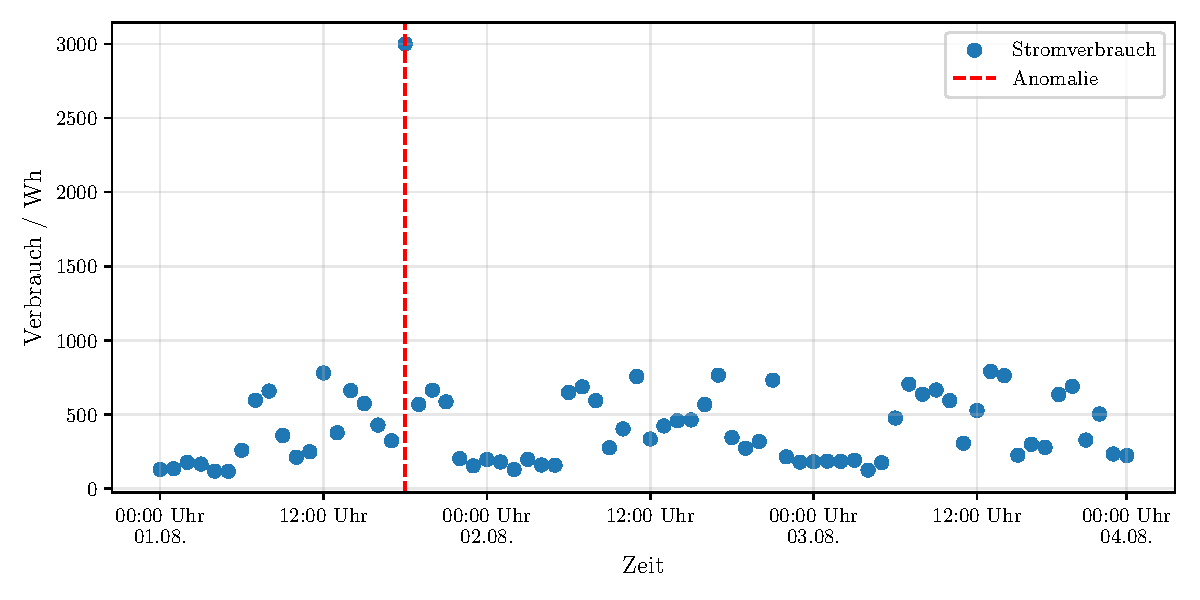
\includegraphics[width=\linewidth]{ch5_anomalien/abbildungen/punktanomalie_bsp.pdf}
    \caption{Gemessener Stromverbrauch mit sichtbarer Punktanomalie}
~\label{fig:punktanomalie_bsp}
\end{figure}

\begin{figure}[h]
    \centering
    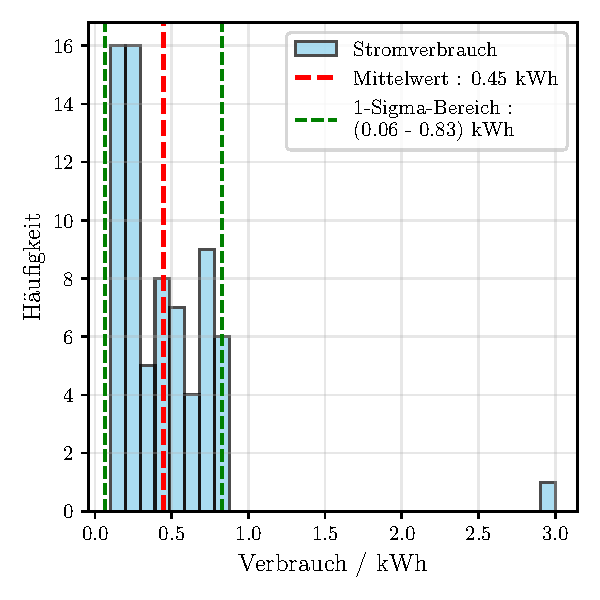
\includegraphics[width=\linewidth]{ch5_anomalien/abbildungen/punktanomalie_hist.pdf}
    \caption{\centering Histogramm des gemessenen Stromverbrauchs}
~\label{fig:punktanomalie_hist}
\end{figure}